\bluepage{Příprava bufferů}

\begin{frame}
\frametitle{Buffery}
  \begin{itemize}
  \item Buffer je objekt zastřešující lineární paměť na GPU
  \item Může obsahovat jakákoliv data
  \item Nejčastěji se používá pro uložení vrcholů geometrie (a jejich vlastností), indexů na vrcholy a materiálů
  \item Buffer lze připojit na několik přípojných míst OpenGL pipeline (binding points)
  \item Binding point udává sémantiku bufferu
  \item Pro vrcholy se používá \textcolor{red}{GL\_ARRAY\_BUFFER}, buffer se pak nazývá Vertex Buffer Object (VBO)
  \item Pro indexy se používá \textcolor{red}{GL\_ELEMENT\_ARRAY\_BUFFER}, Element Buffer Object (EBO)
  \item Pro obecná data se používá \textcolor{red}{GL\_SHADER\_STORAGE\_BUFFER}
  \end{itemize}
\end{frame}

\begin{frame}
\frametitle{OpenGL 4.3 pipeline}
  \begin{figure}[h]
  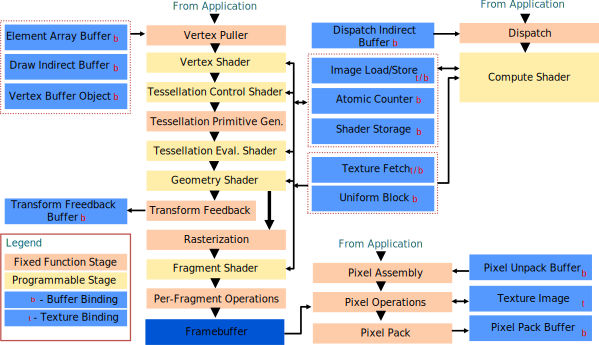
\includegraphics[width=10cm,keepaspectratio]{pics/opengl43_2.pdf}
  \end{figure}
\end{frame}

\begin{frame}[fragile]
\frametitle{Vytvoření buffer, nahrání dat}
    {\scriptsize
    \begin{minted}[frame=lines]{c++}
float data[]={1,2};//data, ktera budeme vkladat do bufferu
GLuint vbo;//identifikator VBO
glGenBuffers(1,&vbo);//vygenerujeme si identifikator
glBindBuffer(GL_ARRAY_BUFFER,vbo);//aktivujeme a vytvorime VBO
//alokujeme buffer a nahrajeme do nej data
glBufferData(GL_ARRAY_BUFFER,sizeof(data),data,GL_STATIC_DRAW);
    \end{minted}
    }
    Změna dat ve VBO.
    {\scriptsize
    \begin{minted}[frame=lines]{c++}
float*ptr;//ukazatel na data
glBindBuffer(GL_ARRAY_BUFFER,vbo);
ptr=(float*)glMapBuffer(GL_ARRAY_BUFFER,GL_READ_WRITE);//namapujeme buffer
ptr[0]=0.5;//nastavime hodnotu prvniho prvku
glUnmapBuffer(GL_ARRAY_BUFFER);//odmapujeme buffer, komitujeme zmeny do GPU
    \end{minted}
    }
    Nebo pomoci {\color{blue} glBufferSubData}.
    {\scriptsize
    \begin{minted}[frame=lines]{c++}
glBufferSubData(GL_ARRAY_BUFFER,
  sizeof(float),//nahrajeme nova s offsetem jeden float
  sizeof(float),//nahrajeme jen jeden float
  data);//data
    \end{minted}
    }
\end{frame}


